% Search for XXXX for places which you need to add your contributions. 

\documentclass{article}
\usepackage{graphicx}

\title{COMP20010 Lab Six: Algorithm Analysis}
\author{Thomas Swann}

\begin{document}
\maketitle

% LAB 6 PART 1
\section{Part~1 Algorithm}
\label{sec:algorithm1}

\subsection{Asymptotic run-time analysis}

My algorithm runs in asymptotic time $O(wN)$. The argument for this follows:

In my program I implemented the Radix Sort algorithm. Radix Sort is a non-comparitive integer sorting algorithm that sorts the data by grouping the elements with the same significant position. After grouping the elements it uses a bucket to reorder the elemements into the correct group. It does this as many times as the longest element. This means that the time complexity is $O(wN)$ where \textit{w} is the length of the largest integer. This is because it does \textit{w} passes and in each pass it looks at all N elements.

\subsection{Experiments}
\label{sec:experiments1}
For my experiments I used the time command for each size of datafile. I then put this data in a data.dat file and used the gnuplot scripts given to plot a graph and fit an equation to the data. I also used "fitscript.p" to find a possible equation to test against. Here are the results:

% If you put your results in a graph, uncomment the following. 

 \begin{figure}
   \centering
 \resizebox{0.9\textwidth}{!}{\includegraphics{my-plot.ps}}  
 
   \caption{Plot of my runtimes}
   \label{fig:experiment1}
 \end{figure}

% If you put your results in a table, the followin might be helpful. 
% Replace the formula in the third column with the formula you are testing. 

 \begin{center}
 \begin{tabular}{l||l|l|}
   data size   & run time    & $t = 4.39\times 10^{-7} \times N$ \\  \hline
   10          & 0.001s      & 0.00000439s  \\
   100         & 0.001s      & 0.0000439s  \\
   1000        & 0.002s      & 0.000439s  \\
   10000       & 0.006s      & 0.00439s  \\
   100000      & 0.046s      & 0.0439s  \\
   1000000     & 0.441s      & 0.439s  \\
   2000000     & 0.878s      & 0.878s  \\
   3000000     & 1.344s      & 1.317s  \\
   4000000     & 1.748s      & 1.756s  \\
   5000000     & 2.206s      & 2.195s  \\
   6000000     & 2.622s      & 2.634s  \\
   7000000     & 3.106s      & 3.073s  \\
   8000000     & 3.503s      & 3.512s  \\
   9000000     & 3.953s      & 3.951s  \\
   10000000    & 4.379s      & 4.390s  \\

 \end{tabular}
 \end{center}

\subsection{Prediction}
\label{sec:prediction1}

My estimate of the equation for the run-time of the algorithm is:
\begin{equation}
  \label{eq:estimated_runtime1}
  t(N) = 4.39\times10^{-7}\times N
\end{equation}
Using this, the estimated time to find the ninetieth percentile of a
file containing 60 million numbers is 26.34 seconds. After running the program 
with a datafile of size 60 million the time recorded was 26.262s which confirms
my prediction.


%LAB 6 PART 2
\section{Part~2 Algorithm}
\label{sec:algorithm2}

\subsection{Asymptotic run-time analysis}

My algorithm runs in asymptotic time $O(wN)$. 

The argument for this follows:
As my program before had a time complexity of $O(wN)$ I didn't change the algorithm used, therefore my reasoning is the same. I did improve the program to make it more efficient. Using the knowledge of how big the numbers will be I removed the part of the program that finds the largest integer and instead did a known number of passes. This obviously will slow the program down for small numbers of N however when doing the experiments the program executed too fast to notice.

\subsection{Experiments}
\label{sec:experiments2}
I tested the program using the same method as before, however when I plotted the graph I used the "plot2data.p" script (data1.dat is the more efficient program and data2.dat is the previous program). Here are the results:

% If you put your results in a graph, uncomment the following. 

 \begin{figure}
   \centering
 \resizebox{0.9\textwidth}{!}{\includegraphics{my-plot3.ps}}  
  
   \caption{A comparison of both programs}
   \label{fig:experiment1}
 \end{figure}

% If you put your results in a table, the followin might be helpful. 
% Replace the formula in the third column with the formula you are testing. 

 \begin{center}
 \begin{tabular}{l||l|l|}
   data size   & run time    & $t = 4.29 \times 10^{-7} \times N$ \\  \hline
   10          & 0.001s       & 0.00000429s \\
   100         & 0.001s       & 0.0000429s \\
   1000        & 0.002s       & 0.000429s \\
   10000       & 0.006s       & 0.00429s \\
   100000      & 0.045s       & 0.0429s \\
   1000000     & 0.433s       & 0.429s  \\
   2000000     & 0.863s       & 0.858s \\
   3000000     & 1.289s       & 1.287s \\
   4000000     & 1.729s       & 1.716s \\
   5000000     & 2.148s       & 2.145s \\
   6000000     & 2.584s       & 2.574s \\
   7000000     & 3.011s       & 3.003s \\
   8000000     & 3.429s       & 3.432s \\
   9000000     & 3.865s       & 3.861s \\
   10000000    & 4.282s       & 4.290s \\

 \end{tabular}
 \end{center}

\subsection{Prediction}
\label{sec:prediction2}

My estimate of the equation for the run-time of the algorithm is:
\begin{equation}
  \label{eq:estimated_runtime2}
  t(N) = 4.29\times10^{-7}\times N
\end{equation}
Using this, the estimated time to find the ninetieth percentile of a
file containing 60 million numbers is 25.74 seconds. After running the program 
with a datafile of size 60 million the time recorded was 25.770s which confirms
my prediction.



\end{document}
